\documentclass[11pt, a4paper]{article}

% ─── Packages ───
\usepackage[margin=2cm]{geometry}
\usepackage{graphicx}
\usepackage{xcolor}
\usepackage{titlesec}
\usepackage{enumitem}
\usepackage{booktabs}
\usepackage{tabularx}
\usepackage{longtable}
\usepackage{multirow}
\usepackage{hyperref}
\usepackage{fancyhdr}
\usepackage{tikz}
\usepackage{fontenc}
\usepackage{parskip}
\usepackage{makecell}
\usepackage{amssymb}
\usepackage{pifont}
\usepackage{float}
\usepackage{array} % Added for raggedright in table columns

\usetikzlibrary{shapes.geometric, arrows.meta, positioning, fit, backgrounds, calc}

% ─── Colors ───
\definecolor{ekagold}{HTML}{D4A843}
\definecolor{ekadark}{HTML}{1A1A2E}
\definecolor{ekagray}{HTML}{333333}
\definecolor{ekaaccent}{HTML}{3B82F6}
\definecolor{sectionblue}{HTML}{1E3A5F}

% Professional Palette for Diagram & UI Elements
\definecolor{coreblue}{HTML}{1E3A8A} % Deep Navy
\definecolor{coregray}{HTML}{475569} % Slate
\definecolor{lightbg}{HTML}{F8FAFC}  % Very light slate
\definecolor{bordergray}{HTML}{CBD5E1} % Light border

% Diagram specific palette
\definecolor{layerclient}{HTML}{1E293B} % Slate 800
\definecolor{layerproto}{HTML}{334155}  % Slate 700
\definecolor{layerserver}{HTML}{475569} % Slate 600
\definecolor{layeragent}{HTML}{1D4ED8}  % Blue 700
\definecolor{layerai}{HTML}{4338CA}     % Indigo 700
\definecolor{layerdb}{HTML}{0F766E}     % Teal 700

% ─── Formatting ───
\titleformat{\section}{\Large\bfseries\color{sectionblue}}{}{0em}{}[\titlerule]
\titleformat{\subsection}{\large\bfseries\color{ekagray}}{}{0em}{}

\hypersetup{
    colorlinks=true,
    linkcolor=ekaaccent,
    urlcolor=ekaaccent,
}

\pagestyle{fancy}
\fancyhf{}
\fancyhead[L]{\small\textcolor{ekagray}{\textbf{EKALAVYA 2.0}}}
\fancyhead[R]{\small\textcolor{ekagray}{Agentic Career Intelligence Platform}}
\fancyfoot[C]{\thepage}
\renewcommand{\headrulewidth}{0.4pt}

% ─── Document ───
\begin{document}

% ─── Title ───
\begin{center}
    {\Huge\bfseries\textcolor{sectionblue}{EKALAVYA 2.0}}\\[4pt]
    {\LARGE\textcolor{ekagray}{Agentic Career Intelligence Platform}}\\[2pt]
    \rule{0.5\textwidth}{0.5pt}
\end{center}

\vspace{6pt}

% ══════════════════════════════════════════════════════════════
\section{Problem Statement}
% ══════════════════════════════════════════════════════════════

\begin{enumerate}[leftmargin=1.5em, itemsep=2pt, label=\textbf{\arabic*.}]
    \item \textbf{The Education--Employment Gap.} Entry-level jobs demand real-world experience, but students graduate with only theoretical knowledge. There is no structured bridge that converts academic learning into demonstrable, recruiter-ready project work.

    \item \textbf{Rote Learning vs.\ Project-Based Learning.} Current platforms teach through passive video lectures and multiple-choice assessments. Students need guided, phase-wise project building --- from environment setup to deployment with AI mentorship at every step, not just answers handed to them.

    \item \textbf{No Single Platform Does It All.} Today, a student must juggle 5--6 different tools: one for resume analysis, another for learning, a separate IDE for coding, a different app for collaboration, yet another for job searching. There is no unified platform where a student can analyse their skills, get guided projects, build them in a live collaborative workspace with peers, and get matched to jobs --- all in one place.
\end{enumerate}

% ══════════════════════════════════════════════════════════════
\section{Our Solution}
% ══════════════════════════════════════════════════════════════

\textbf{Ekalavya} is a unified agentic career platform that directly addresses each gap:

\begin{itemize}[leftmargin=1.5em, itemsep=2pt]
    \item \textbf{Bridging the Experience Gap:} Students can describe their project interests or simply upload their resume. AI extracts their current skills, identifies gaps against their target role, and generates personalised projects on various difficulty levels that build exactly the missing competencies. Completed projects feed directly into their lab and progress is recorded.

    \item \textbf{Structured Project-Based Learning:} Every project follows a 6-phase guided roadmap (Setup $\rightarrow$ Core Logic $\rightarrow$ Database $\rightarrow$ API $\rightarrow$ Frontend $\rightarrow$ Deployment). An AI mentor coaches students through each phase inside a full in-browser IDE. It teaches, hints, and verifies. The AI can autonomously update code and unlock the next phase only when the current one is genuinely complete.

    \item \textbf{Everything in One Place:} Resume analysis, AI career coaching, a Monaco-powered code editor, live multiplayer collaboration (via 6-digit session codes) where like-minded people can brainstorm in one common workspace, community discussion channels, academic research tools, skill-delta job matching, and progress tracking, all inside a single application, connected through a unified agentic backend.
\end{itemize}

\vspace{6pt}
\noindent\textbf{The Novelty Factor:} The real breakthrough of Ekalavya 2.0 is that the AI isn't just a chatbot that gives text answers it is an active co-developer with actual control over your environment. If a student gets stuck, the AI mentor can directly edit code in their in-browser IDE, run terminal commands, and physically demonstrate fixes. Furthermore, it introduces "AI-Assisted Collaboration": you and your friends can join the same live coding session, writing code together while a shared AI mentor guides the entire group. No other platform combines live collaborative coding with AI agents that can actually take action inside the workspace.

\newpage

% ══════════════════════════════════════════════════════════════
\section{System Architecture}
% ══════════════════════════════════════════════════════════════

The platform is built on the \textbf{Model Context Protocol (MCP)}, an open standard where every user interaction is a structured AI tool call. This makes the system inherently agentic: the AI layer doesn't just respond, it takes actions.

\begin{figure}[H]
\centering
\resizebox{\textwidth}{!}{
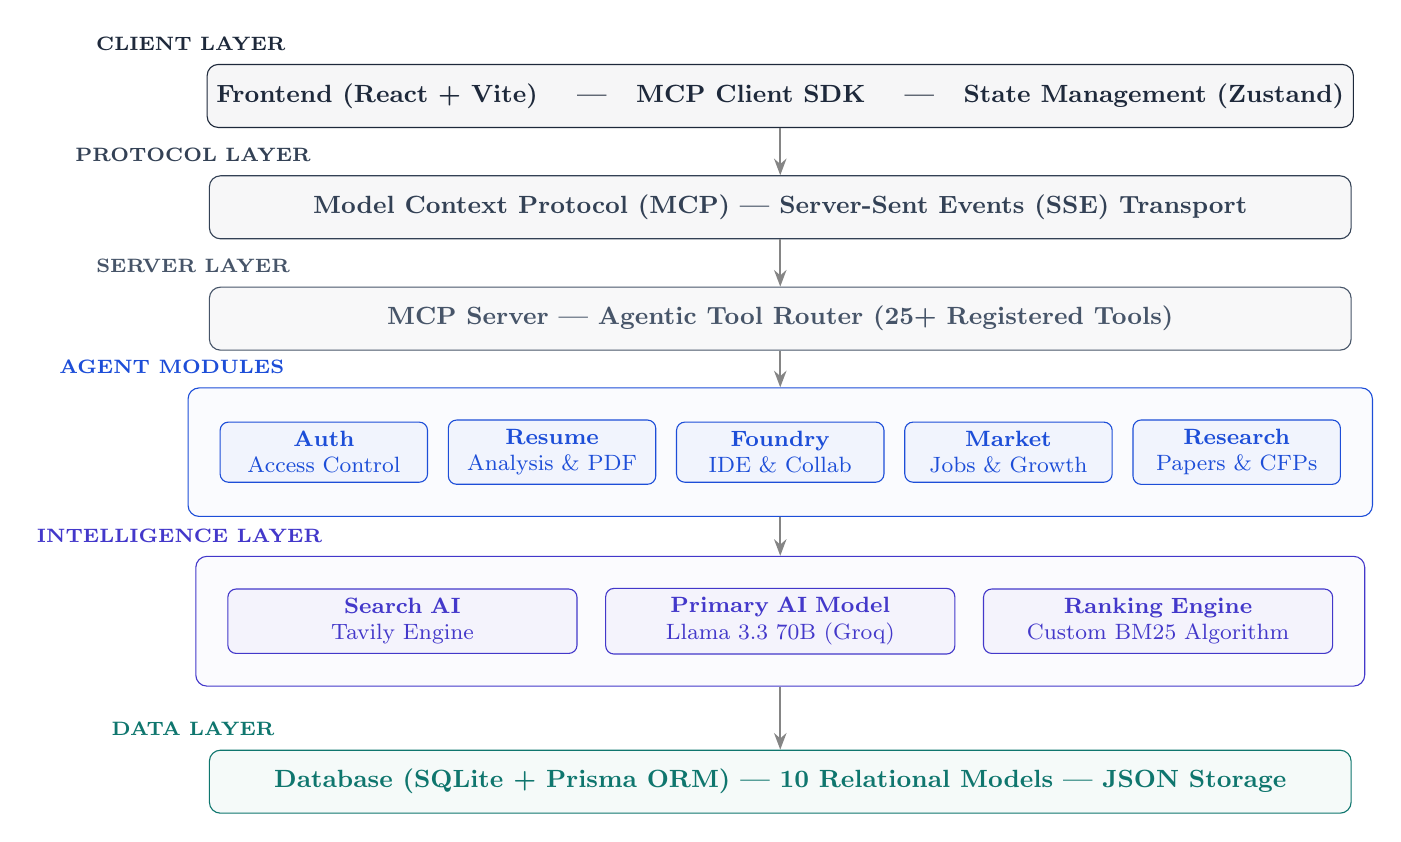
\begin{tikzpicture}[
    node distance=0.5cm,
    layer/.style={rectangle, rounded corners=4pt, draw=#1, fill=#1!4, minimum width=14.5cm, minimum height=0.8cm, align=center, font=\small\bfseries, text=#1},
    sublayer/.style={rectangle, rounded corners=3pt, draw=#1, fill=#1!6, minimum height=0.7cm, align=center, font=\footnotesize, text=#1},
    arr/.style={-{Stealth[length=6pt]}, thick, color=ekagray!60},
    layerlabel/.style={font=\scriptsize\bfseries, color=#1, anchor=south west},
]

% ─── Layer 1: Client ───
\node[layer=layerclient] (client) {Frontend (React + Vite) \quad---\quad MCP Client SDK \quad---\quad State Management (Zustand)};
\node[layerlabel=layerclient, above=0.05cm of client.north west, xshift=-0.2cm] {CLIENT LAYER};

% ─── Layer 2: Protocol ───
\node[layer=layerproto, below=0.6cm of client] (proto) {Model Context Protocol (MCP) --- Server-Sent Events (SSE) Transport};
\node[layerlabel=layerproto, above=0.05cm of proto.north west, xshift=-0.2cm] {PROTOCOL LAYER};

% ─── Layer 3: Server ───
\node[layer=layerserver, below=0.6cm of proto] (server) {MCP Server --- Agentic Tool Router (25+ Registered Tools)};
\node[layerlabel=layerserver, above=0.05cm of server.north west, xshift=-0.2cm] {SERVER LAYER};

% ─── Layer 4: Agent Modules (SINGLE HORIZONTAL ROW) ───
\node[sublayer=layeragent, below=0.9cm of server, text width=2.4cm] (foundry) {\textbf{Foundry}\\IDE \& Collab};
\node[sublayer=layeragent, left=0.25cm of foundry, text width=2.4cm] (resume) {\textbf{Resume}\\Analysis \& PDF};
\node[sublayer=layeragent, left=0.25cm of resume, text width=2.4cm] (auth) {\textbf{Auth}\\Access Control};
\node[sublayer=layeragent, right=0.25cm of foundry, text width=2.4cm] (market) {\textbf{Market}\\Jobs \& Growth};
\node[sublayer=layeragent, right=0.25cm of market, text width=2.4cm] (research) {\textbf{Research}\\Papers \& CFPs};

\begin{scope}[on background layer]
\node[rectangle, rounded corners=4pt, draw=layeragent, fill=layeragent!2,
      fit=(auth)(resume)(foundry)(market)(research),
      inner xsep=0.4cm, inner ysep=0.4cm] (agentbox) {};
\end{scope}
\node[layerlabel=layeragent, above=0.05cm of agentbox.north west, xshift=-0.2cm] {AGENT MODULES};

% ─── Layer 5: AI Models (SINGLE HORIZONTAL ROW) ───
\node[sublayer=layerai, below=0.9cm of agentbox, text width=4.2cm] (model1) {\textbf{Primary AI Model}\\Llama 3.3 70B (Groq)};
\node[sublayer=layerai, left=0.35cm of model1, text width=4.2cm] (model2) {\textbf{Search AI}\\Tavily Engine};
\node[sublayer=layerai, right=0.35cm of model1, text width=4.2cm] (model3) {\textbf{Ranking Engine}\\Custom BM25 Algorithm};

\begin{scope}[on background layer]
\node[rectangle, rounded corners=4pt, draw=layerai, fill=layerai!2,
      fit=(model1)(model2)(model3),
      inner xsep=0.4cm, inner ysep=0.4cm] (aibox) {};
\end{scope}
\node[layerlabel=layerai, above=0.05cm of aibox.north west, xshift=-0.2cm] {INTELLIGENCE LAYER};

% ─── Layer 6: Database ───
\node[layer=layerdb, below=0.8cm of aibox] (db) {Database (SQLite + Prisma ORM) --- 10 Relational Models --- JSON Storage};
\node[layerlabel=layerdb, above=0.05cm of db.north west, xshift=-0.2cm] {DATA LAYER};

% ─── Arrows ───
\draw[arr] (client) -- (proto);
\draw[arr] (proto) -- (server);
\draw[arr] (server) -- (agentbox);
\draw[arr] (agentbox) -- (aibox);
\draw[arr] (aibox) -- (db);

\end{tikzpicture}
}
\vspace{-10pt}
\caption{Ekalavya 2.0 --- Hierarchical Software Pipeline \& Agentic Framework}
\end{figure}

\vspace{10pt}

% ══════════════════════════════════════════════════════════════
\section{Tech Stack}
% ══════════════════════════════════════════════════════════════

\begin{table}[H]
\centering
\renewcommand{\arraystretch}{1.15}
\begin{tabularx}{\textwidth}{@{}l l X@{}}
\toprule
\textbf{Layer} & \textbf{Technology} & \textbf{Purpose} \\
\midrule
Frontend & React + Vite & UI framework  \\
Styling & Tailwind CSS  & Responsive design with animations \\
Code Editor & Monaco Editor & In-browser IDE \\
Protocol & MCP over SSE & AI-native tool-call communication \\
Backend & TypeScript + MCP Server & Modular agentic tool framework \\
AI & Llama 3.3 70B (via Groq) & Fast inference for 8 AI agent personas \\
Search & Tavily API & Live job listings and conference data \\
Database & SQLite + Prisma ORM & Relational storage with type safety \\
\bottomrule
\end{tabularx}
\end{table}

\newpage

% ══════════════════════════════════════════════════════════════
\section{Platform Features \& AI Pipeline}
% ══════════════════════════════════════════════════════════════

{
\renewcommand{\arraystretch}{1.4} % Add breathing room between rows
\small
\begin{longtable}{@{} 
    >{\raggedright\bfseries}p{3cm} 
    >{\raggedright\bfseries}p{3.5cm} 
    >{\raggedright}p{7cm} 
    >{\raggedright\arraybackslash}p{2.5cm} @{}}
\toprule
\textbf{Feature Module} & \textbf{Tool / Component} & \textbf{What It Does} & \textbf{AI Persona} \\
\midrule
\endfirsthead

\toprule
\textbf{Feature Module} & \textbf{Tool / Component} & \textbf{What It Does} & \textbf{AI Persona (cont.)} \\
\midrule
\endhead

\bottomrule
\endfoot

\bottomrule
\endlastfoot

% --- RESUME INTELLIGENCE ---
\textbf{Resume Intelligence} & Resume Parser & Uploads PDF/TXT resume, extracts full text & --- \\
 & Skill Gap Analysis & Identifies current skills, gaps, and SWOT matrix & Mirror Agent \\
\midrule

% --- THE FOUNDRY ---
\textbf{The Foundry} & Project Generator & Creates 9 personalised projects (Easy / Medium / Hard) & Lab Agent \\
 & 6-Phase Roadmap & Setup $\rightarrow$ Logic $\rightarrow$ DB $\rightarrow$ API $\rightarrow$ UI $\rightarrow$ Deploy & Phase Architect \\
 & Monaco Code Editor & Full multi-file, multi-language IDE in the browser & --- \\
 & AI Mentor Chat & Guide through each phase & Foundry Mentor \\
 & Code Execution & Simulates terminal output & Terminal Emulator \\
 & \textbf{Live Collaboration} & \textbf{6-digit session codes to invite peers into shared workspaces; synchronised code, team chat, and project progress across all participants} & --- \\
\midrule

% --- CAREER INTELLIGENCE ---
\textbf{Career Intelligence} & AI Career Coach & Multi-session chat; reads projects, and progress context & Career Mentor \\
 & Dashboard Architect & Describe a vision in plain text $\rightarrow$ get a full project blueprint & Dashboard Architect \\
\midrule

% --- MARKET & JOBS ---
\textbf{Market \& Jobs} & Job Matching & Skill-delta matching against live LinkedIn/Glassdoor listings & Job Scout \\
 & Activity Heatmap & GitHub-style 365-day learning contribution tracker & --- \\
\midrule

% --- RESEARCH & COMMUNITY ---
\textbf{Research \& \newline Community} & Paper Search & Google Scholar scraping for search & --- \\
 & Conference Tracker & Upcoming conferences deadlines & --- \\
 & Community Channels & Categorised discussion forums with real-time chat sync & --- \\

\end{longtable}
}

\vspace{10pt}

% ══════════════════════════════════════════════════════════════
\section{Target Audience \& Impact}
% ══════════════════════════════════════════════════════════════

\begin{table}[H]
\centering
\renewcommand{\arraystretch}{1.3}
\begin{tabularx}{\textwidth}{@{} >{\bfseries}p{4.5cm} X @{}}
\toprule
\textbf{User Segment} & \textbf{Core Value Proposition} \\
\midrule
University Students & Bridges the gap between theoretical coursework and practical, recruiter-ready project portfolios. \\
Self-Taught Developers & Provides autonomous AI mentorship and structured roadmaps missing from self-paced video tutorials. \\
Peer Study Groups & Enables live collaborative coding (multiplayer mode) in a shared browser-based workspace. \\
\bottomrule
\end{tabularx}
\end{table}

\newpage

% ══════════════════════════════════════════════════════════════
\section{Competitive Landscape \& USP}
% ══════════════════════════════════════════════════════════════

Ekalavya 2.0 introduces a paradigm shift by combining the best elements of learning, coding, and AI into a single agentic workflow, dramatically outperforming fragmented traditional tools.

\begin{table}[H]
\centering
\renewcommand{\arraystretch}{1.4}
\small
\begin{tabularx}{\textwidth}{@{} >{\bfseries}p{2.6cm} p{2.8cm} p{3.2cm} p{2.8cm} >{\bfseries\color{sectionblue}}X @{}}
\toprule
\textbf{Aspect} & \textbf{Traditional EdTech} (Udemy, Coursera) & \textbf{Coding Platforms} (LeetCode, HackerRank) & \textbf{Standard AI} (ChatGPT, Claude) & \textbf{Ekalavya 2.0} (Our USP) \\
\midrule
Learning Method & Passive video lectures \& quizzes & Solo puzzle-solving \& algorithms & Text-based Q\&A & Phase-wise, agent-mentored full project building \\
Workspace & None (Requires local environment setup) & Basic text editor in browser & No execution environment & Full browser IDE (Monaco) with AI environment control \\
Collaboration & Solo learning & Solo practice & Solo interaction & Live multiplayer coding with a shared AI mentor \\
Career Alignment & Generic certificates & Generic interview prep & Generic advice & Auto-generates projects based on exact resume skill gaps \\
\bottomrule
\end{tabularx}
\end{table}

\vspace{10pt}

% ══════════════════════════════════════════════════════════════
\section{Plans Ahead}
% ══════════════════════════════════════════════════════════════

\begin{enumerate}[leftmargin=1.5em, itemsep=4pt, label=\textbf{\arabic*.}]

    \item \textbf{Deep Native Workspace Expansion.}
    Evolving the in-browser workspace into a production-grade development environment --- with real sandboxed code execution (Docker), integrated version control, multi-file debugging, and full terminal access. The goal is to support real-world, heavy software engineering workflows, not just learning exercises.

    \item \textbf{Intelligent Agentic Research Layer.}
    Building a dedicated research pipeline that doesn't blindly abuse the AI model's capability but will intelligently fetch and cross-reference data from research papers, technical articles, open-source repositories, and official documentation then synthesise that knowledge into highly accurate, framework-based, phase-wise project blueprints.

    \item \textbf{Standalone Local CLI Tooling.}
    Packaging the entire platform as an individual, laptop-installable CLI tool. Students will be able to run the full agentic workflow natively on their machines personalising the whole experience.

    \item \textbf{Enterprise-Grade Security Layer.}
    Implementing end-to-end authentication with encrypted sessions, role-based access control, secure API key management, and sandboxed code execution isolation. Every collaborative session, AI interaction, and data transfer will be secured to enterprise standards making the platform viable for institutional and corporate deployment.

\end{enumerate}

\vspace{30pt}

% ─── Demo Link Provision ───
\begin{center}
    \fcolorbox{bordergray}{lightbg}{
        \parbox{0.8\textwidth}{
            \centering
            \vspace{6pt}
            \textbf{\Large\textcolor{coreblue}{Demo Video}} \\[6pt]
            \href{https://drive.google.com/file/d/17Xai16W3YMP_vJrZZUiQqdskJKBh9xHu/view?usp=sharing}{\textcolor{ekaaccent}{\underline{Click here to view the demo}}}
            \vspace{6pt}
        }
    }
\end{center}

\end{document}
